\documentclass[11pt]{article}

\usepackage{amsmath,amssymb,mathtools}
\usepackage[margin=1in]{geometry}
\usepackage{enumitem}
\usepackage{xcolor}
\usepackage{microtype}
\usepackage{graphicx}
\usepackage{tikz,float}
\usepackage{subcaption}
\usepackage{amsthm}
\usepackage{hyperref}
\usepackage{array}
\usepackage{pgfplots}

\usetikzlibrary{shapes.geometric, arrows.meta, positioning, calc, decorations.markings}
\tikzset{
	block/.style={rectangle, draw, text width=6em, text centered, rounded corners, minimum height=10mm},
	sum/.style={circle, draw, node distance=1.5cm},
	line/.style={draw, -{Stealth[length=2.5mm, width=1.5mm]}}
}

\usepgfplotslibrary{groupplots}
\pgfplotsset{compat=1.18}

\pgfplotsset{
	myaxes/.style={
		axis lines=middle,
		axis line style={-latex},
		grid=major,
		grid style={gray!15},
		minor grid style={gray!35},
		xlabel style={at={(ticklabel* cs:1)}, anchor=north west},
		ylabel style={at={(ticklabel* cs:1)}, anchor=south east},
		every axis plot/.append style={thick}
	},
	myplotstyle/.style={
		width=14cm,
		height=7cm,
		axis lines=middle,
		axis line style={-Stealth},
		grid=both,
		minor tick num=1,
		major grid style={draw=gray!30},
		minor grid style={draw=gray!15},
		tick label style={font=\small, fill=white, inner sep=1.5pt},
		xlabel={$t$},
		ylabel={$x(t)$},
		xlabel style={anchor=north east, font=\small},
		ylabel style={anchor=south east, font=\small},
		samples=401,
	}
}

\newtheoremstyle{mynote}
{6pt}      % Space above
{6pt}      % Space below
{}          % Body font (normal, not italic)
{}          % Indent amount
{\bfseries} % Theorem head font
{.}         % Punctuation after theorem head
{.5em}      % Space after theorem head
{}          % Theorem head spec
\theoremstyle{mynote}
\newtheorem{definition}{Definition}
\newtheorem{proposition}{Proposition}
\newtheorem{example}{Example}
\newtheorem{remark}{Remark}
\newtheorem{theorem}{Theorem}
\newtheorem{corollary}{Corollary}

\newcommand{\T}{\mathcal{T}}
\newcommand{\R}{\mathbb{R}}
\newcommand{\Z}{\mathbb{Z}}
\newcommand{\C}{\mathbb{C}}
\newcommand{\conv}{\ast}
\newcommand{\dt}{\,\dd t}
\newcommand{\dd}{\mathrm{d}}
\newcommand{\imp}{\delta}
\newcommand{\sinc}[1]{\frac{\sin(\pi #1)}{\pi #1}}


\DeclareMathOperator{\rect}{rect}
\DeclareMathOperator{\Ev}{Ev}
\DeclareMathOperator{\Od}{Od}
\DeclareMathOperator{\sgn}{sgn}
\DeclareMathOperator{\step}{u}
\DeclareMathOperator{\tri}{tri}



\begin{document}
	% Reset figure counter for this lecture
	\renewcommand{\thefigure}{10.\arabic{figure}}
	
	% --- TITLE BLOCK ---
	\thispagestyle{empty}
	\noindent
	\begin{tabular*}{\textwidth}{l @{\extracolsep{\fill}} r}
		\textbf{Signals and Systems} & \textbf{Lecture 10} \\
		\textit{Dr. Ghandi Manasra and Ahmed Rabei} & \textit{Fall 2025} \\
	\end{tabular*}
	\hrule
	\vspace{0.4cm}
	\begin{center}
		\Large\textbf{Lecture 10: LTI Systems \& Filtering}
	\end{center}
	\vspace{0.4cm}
	
	\section*{Reference}
	Oppenheim \& Willsky, \textit{Signals and Systems}, Chapter 3, Sections 3.8--3.11
	
	\section*{Review of Lecture 9}
	\begin{itemize}[noitemsep]
		\item DTFS as finite sum representation
		\item Orthogonality of discrete-time harmonics
		\item Parseval's relation for periodic signals
		\item Multiplication and circular convolution
	\end{itemize}
	
	\section*{10.1 Introduction}
	
	Last time, we completed our foundation in Fourier series by developing the \textbf{Discrete-Time Fourier Series (DTFS)}. We discovered that any periodic discrete-time signal can be represented as a finite sum of harmonically related complex exponentials, and we explored the properties that make this representation so powerful.
	
	Today, we will combine everything we've learned about LTI systems and Fourier series to understand how LTI systems respond to periodic inputs. This leads us to one of the most important applications in signal processing: \textbf{filtering}. We will see that the complex exponential eigenfunction property we discovered earlier makes the analysis of LTI systems with periodic inputs remarkably simple.
	
	The key insight is that when we input a complex exponential to an LTI system, the output is simply a scaled version of the same exponential. This means that if we represent a periodic input as a sum of complex exponentials (using Fourier series), the output can be found by scaling each component by the system's frequency response.
	
	\section*{10.2 The Response of LTI Systems to Complex Exponentials}
	
	 \textbf{LTI systems have a particularly simple response to complex exponential inputs}. When we input a complex exponential signal $x(t) = e^{j\omega t}$ to an LTI system with impulse response $h(t)$, the output is:
	
	\begin{theorem}
		For a continuous-time LTI system with impulse response $h(t)$:
		\[
		x(t) = e^{j\omega t} \rightarrow y(t) = H(j\omega) e^{j\omega t}
		\]
		where $H(j\omega)$ is the \textbf{frequency response} of the system, defined as:
		\[
		H(j\omega) = \int_{-\infty}^{\infty} h(\tau) e^{-j\omega\tau} \dd\tau
		\]
	\end{theorem}
	
	\textbf{Note:} This eigenfunction property and the definition of the frequency response $H(j\omega)$ were first introduced and derived in Lecture 7, Section 7.2.
	
	This means that complex exponentials are \textbf{eigenfunctions} of LTI systems - they maintain their functional form while being scaled by the complex number $H(j\omega)$.
	
	\begin{figure}[H]
		\centering
		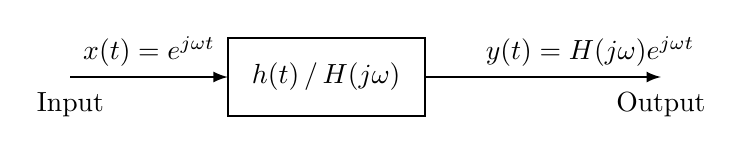
\begin{tikzpicture}[>=latex]
	% Define important coordinates
	\coordinate (input) at (0,0);
	\coordinate (block_left) at (2,-0.5);
	\coordinate (block_right) at (4.5,0.5);
	\coordinate (system_center) at (3.25,0); % Slightly left for visual balance
	\coordinate (output) at (7.5,0);
	
	% Draw main system block (wider, taller)
	\draw[thick] (block_left) rectangle (block_right);
	\node at (system_center) {$h(t)\,/\,H(j\omega)$};
	
	% Arrows and input/output signals
	\draw[->, thick] (input) -- (2,0) node[midway, above] {$x(t) = e^{j\omega t}$};
	\draw[->, thick] (4.5,0) -- (output) node[pos=0.7, above] {$y(t) = H(j\omega)e^{j\omega t}$}; % <-- changed pos=0.7
	
	% Labels for input and output
	\node[below=2pt] at (input) {Input};
	\node[below=2pt] at (output) {Output};
\end{tikzpicture}

		\label{fig:lti_response}
	\end{figure}
	 
	\section*{10.3 Fourier Series and LTI Systems}
	
	When we have a periodic input signal represented by its Fourier series:
	\[
	x(t) = \sum_{k=-\infty}^{\infty} a_k e^{jk\omega_0 t}
	\]
	
	The output of an LTI system becomes:
	\[
	y(t) = \sum_{k=-\infty}^{\infty} a_k H(jk\omega_0) e^{jk\omega_0 t}
	\]
	
	\begin{proposition}
		For a periodic input with Fourier coefficients $a_k$, the output coefficients are:
		\[
		b_k = a_k H(jk\omega_0)
		\]
		The same relationship holds for discrete-time systems:
		\[
		b_k = a_k H(e^{jk(2\pi/N)})
		\]
	\end{proposition}
	
	\begin{definition}[Discrete-Time Frequency Response]
		For a discrete-time LTI system with impulse response $h[n]$, the frequency response is defined as:
		\[
		H(e^{j\omega}) = \sum_{n=-\infty}^{\infty} h[n] e^{-j\omega n}
		\]
	\end{definition}
	
	\textbf{Key Insight:} Each Fourier coefficient $a_k$ is multiplied by the system's frequency response at that harmonic frequency $H(jk\omega_0)$. This allows us to predict exactly how the system will modify each frequency component of the input signal.

	\section*{10.4 The Concept of Filtering}
	
	The relationship $b_k = a_k H(jk\omega_0)$ tells us that an LTI system can change the magnitude and phase of each frequency component of a signal. This process is called \textbf{filtering}.
	
	\begin{definition}
		Filtering is the process of selectively emphasizing or attenuating different frequency components of a signal.
	\end{definition}
	
	\subsection*{10.4.1 Types of Filters}
	
	We can classify filters based on what they do to the frequency spectrum:
	
	\begin{itemize}[noitemsep]
		\item \textbf{Frequency-Shaping Filters:} These filters alter the overall shape of the spectrum.
		\item \textbf{Frequency-Selective Filters:} These are designed to pass certain frequencies and reject others.
		\begin{itemize}[noitemsep]
			\item \textbf{Lowpass Filter:} Passes low frequencies, rejects high frequencies.
			\item \textbf{Highpass Filter:} Passes high frequencies, rejects low frequencies.
			\item \textbf{Bandpass Filter:} Passes a specific band of frequencies.
		\end{itemize}
	\end{itemize}
	
	\begin{figure}[H]
		\centering
		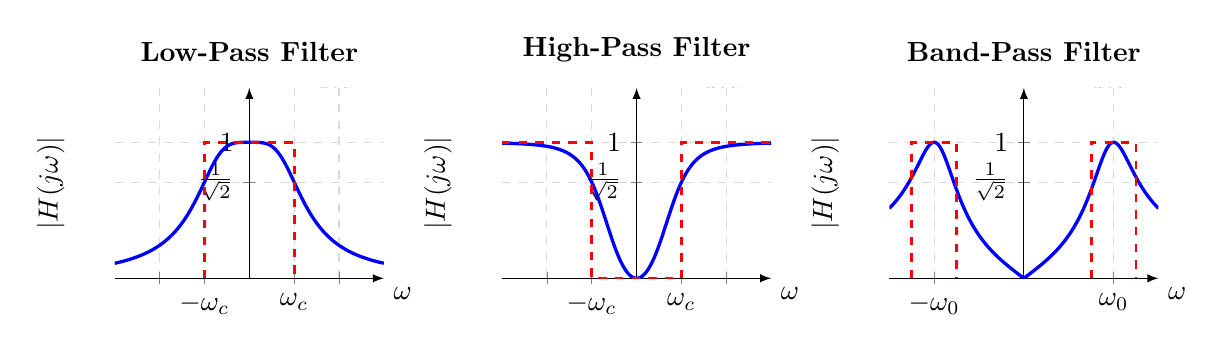
\begin{tikzpicture}
	\begin{groupplot}[
		group style={
			group size=3 by 1,
			horizontal sep=1.5cm,
			vertical sep=0.5cm
		},
		myaxes,
		width=5cm,
		height=4cm,
		xlabel={\(\omega\)},
		ylabel={\(|H(j\omega)|\)},
ylabel style={at={(axis description cs:-0.15,0.5)}, anchor=south, rotate=90},
		ymin=0, ymax=1.4,
		xmin=-3, xmax=3,
		xtick={-2, -1, 0, 1, 2},
		xticklabels={, \(-\omega_c\), 0, \(\omega_c\),},
		ytick={0, 0.707, 1},
		yticklabels={0, \(\frac{1}{\sqrt{2}}\), 1},
		domain=-3:3,
		samples=300,
		every axis plot/.append style={thick, no marks},
		grid=major,
		grid style={dashed, gray!30}
		]
		
		% Low-pass filter (2nd-order Butterworth)
		\nextgroupplot[title={\textbf{Low-Pass Filter}}]
		\addplot[blue, line width=1.2pt] {1/sqrt(1+x^4)};
		\addplot[red, dashed, line width=1pt] coordinates {(-1,0) (-1,1) (1,1) (1,0)};
		\node[anchor=south east, font=\small] at (rel axis cs:0.95,0.95) {Ideal};
		
		% High-pass filter (2nd-order Butterworth)
		\nextgroupplot[title={\textbf{High-Pass Filter}}]
		\addplot[blue, line width=1.2pt] {(x^2)/sqrt(1+x^4)};
		\addplot[red, dashed, line width=1pt] coordinates {(-3,1) (-1,1) (-1,0) (0,0) (1,0) (1,1) (3,1)};
		\node[anchor=south east, font=\small] at (rel axis cs:0.95,0.95) {Ideal};
		
		% Band-pass filter (Improved resonance)
		\nextgroupplot[
		title={\textbf{Band-Pass Filter}},
		xtick={-2, 0, 2},
		xticklabels={\(-\omega_0\), 0, \(\omega_0\)}
		]
		\addplot[blue, line width=1.2pt] {abs(x)/sqrt((4-x^2)^2 + x^2)};
		\addplot[red, dashed, line width=1pt] coordinates {(-2.5,0) (-2.5,1) (-1.5,1) (-1.5,0)};
		\addplot[red, dashed, line width=1pt] coordinates {(1.5,0) (1.5,1) (2.5,1) (2.5,0)};
		\node[anchor=south east, font=\small] at (rel axis cs:0.95,0.95) {Ideal};
		
	\end{groupplot}
\end{tikzpicture}

		\caption{Ideal filter characteristics showing (a) lowpass, (b) highpass, and (c) bandpass filters}
		\label{fig:filter_types}
	\end{figure}
	
	The range of frequencies a filter passes is its \textbf{passband}. The range it rejects is its \textbf{stopband}. The boundary between them is the \textbf{cutoff frequency}.
	
	\section*{10.5 Practical Filter Implementations}
	
	\subsection*{10.5.1 RC Low-Pass Filter}
	
	The simplest practical low-pass filter is the RC circuit, consisting of a resistor in series with a capacitor. Its transfer function is:
	
	\begin{theorem}[RC Low-Pass Filter]
		For an RC circuit with input voltage $x(t)$ and output voltage $y(t)$ across the capacitor:
		\[
		H(j\omega) = \frac{1}{1 + j\omega RC}
		\]
		
		\textbf{Key characteristics:}
		\begin{itemize}[noitemsep]
			\item \textbf{Cutoff frequency:} $f_c = \frac{1}{2\pi RC}$
			\item \textbf{Magnitude response:} $|H(j\omega)| = \frac{1}{\sqrt{1 + (\omega RC)^2}}$
			\item \textbf{-3dB point:} At the cutoff frequency, the output is reduced to $\frac{1}{\sqrt{2}} \approx 0.707$ of the input
			\item \textbf{Roll-off rate:} 20 dB per decade (6 dB per octave) in the stop band
		\end{itemize}
	\end{theorem}
	
	\begin{figure}[H]
		\centering
		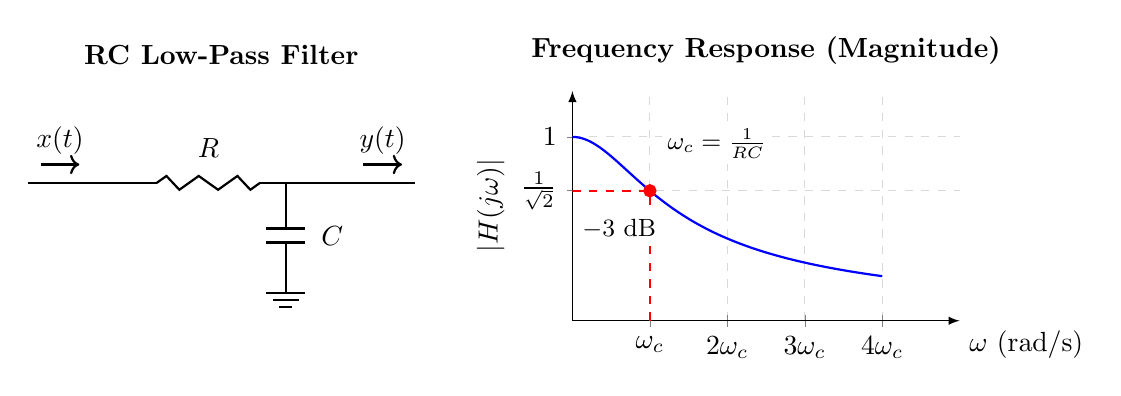
\begin{tikzpicture}
	\begin{groupplot}[
		group style={
			group size=2 by 1,
			horizontal sep=2cm,
			vertical sep=0.5cm
		},
		myaxes,
		width=6.5cm,
		height=4.5cm
		]
		
		% RC Circuit diagram
		\nextgroupplot[
		hide axis,
		title={RC Low-Pass Filter},
		title style={font=\bfseries},
		xmin=0, xmax=6, ymin=-3, ymax=2
		]
		% Input wire
		\draw[thick] (0,0) -- (2,0);
		
		% Resistor (improved zigzag pattern)
		\draw[thick] (2,0) -- (2.15,0.15) -- (2.35,-0.15) -- (2.65,0.15) 
		-- (2.95,-0.15) -- (3.25,0.15) -- (3.45,-0.15) -- (3.6,0);
		\draw[thick] (3.6,0) -- (4,0);
		
		% Connection to capacitor
		\draw[thick] (4,0) -- (4,-1);
		
		% Capacitor (parallel plates)
		\draw[thick, line width=1pt] (3.7,-1) -- (4.3,-1);
		\draw[thick, line width=1pt] (3.7,-1.3) -- (4.3,-1.3);
		\draw[thick] (4,-1.3) -- (4,-2.4);
		
		% Output wire
		\draw[thick] (4,0) -- (6,0);
		
		% Component labels with better positioning
		\node[above] at (2.8,0.35) {$R$};
		\node[right] at (4.4,-1.15) {$C$};
		
		% Input/Output labels with arrows
		\draw[->, thick] (0.2,0.4) -- (0.8,0.4);
		\node[above] at (0.5,0.4) {$x(t)$};
		\draw[->, thick] (5.2,0.4) -- (5.8,0.4);
		\node[above] at (5.5,0.4) {$y(t)$};
		
		% Improved ground symbol
		\draw[thick] (3.7,-2.4) -- (4.3,-2.4);
		\draw[thick] (3.8,-2.55) -- (4.2,-2.55);
		\draw[thick] (3.9,-2.7) -- (4.1,-2.7);
		
		% Frequency response
% Frequency response
\nextgroupplot[
title={Frequency Response (Magnitude)},
title style={font=\bfseries},
xlabel={$\omega$ (rad/s)},
ylabel={$|H(j\omega)|$},
ymin=0, ymax=1.25,
xmin=0, xmax=5,
xtick={0,1,2,3,4},
xticklabels={0,$\omega_c$,$2\omega_c$,$3\omega_c$,$4\omega_c$},
ytick={0,0.707,1},
yticklabels={0,$\frac{1}{\sqrt{2}}$,1},
ylabel style={at={(axis description cs:-0.15,0.5)}, anchor=south, rotate=90},
domain=0:4,
samples=300,
grid=major,
grid style={dashed, gray!30}
]

		% Main frequency response curve
		\addplot[blue, thick, smooth] {1/sqrt(1+x^2)};

		
		% Cutoff frequency marker
		\addplot[red, dashed, thick] coordinates {(1,0) (1,0.707)};
		\addplot[red, dashed, thick] coordinates {(0,0.707) (1,0.707)};
		
		% Cutoff point
		\addplot[red, mark=*, only marks, mark size=2pt] coordinates {(1,0.707)};
		
		% Annotations
		\node[anchor=south west, fill=white, inner sep=2pt] at (axis cs:1.15,0.85) 
		{\small $\omega_c = \frac{1}{RC}$};
		\node[anchor=west, fill=white, inner sep=2pt] at (axis cs:0.05,0.5) 
		{\small $-3$ dB};
		
	\end{groupplot}
\end{tikzpicture}

		\caption{RC low-pass filter circuit and its frequency response characteristics}
		\label{fig:rc_filter}
	\end{figure}
	
	\subsection*{10.5.2 RC High-Pass Filter}
	
	By swapping the positions of the resistor and capacitor, we create a high-pass filter with transfer function:
	\[
	H(j\omega) = \frac{j\omega RC}{1 + j\omega RC}
	\]
	
	This configuration blocks DC and low frequencies while passing high frequencies.
	
	\begin{example}[RC High-Pass Filter Analysis]
		Consider an RC high-pass filter with $R = 1\text{k}\Omega$ and $C = 1\mu\text{F}$. Find the cutoff frequency and analyze the response to a sinusoidal input.
		
		\textbf{Solution:}
		The transfer function is:
		\[
		H(j\omega) = \frac{j\omega RC}{1 + j\omega RC} = \frac{j\omega \cdot 10^3 \cdot 10^{-6}}{1 + j\omega \cdot 10^3 \cdot 10^{-6}} = \frac{j\omega \cdot 10^{-3}}{1 + j\omega \cdot 10^{-3}}
		\]
		
		The cutoff frequency is:
		\[
		f_c = \frac{1}{2\pi RC} = \frac{1}{2\pi \cdot 10^3 \cdot 10^{-6}} = \frac{1}{2\pi \cdot 10^{-3}} = \frac{1000}{2\pi} \approx 159.2 \text{ Hz}
		\]
		
		For an input $x(t) = \cos(2\pi \cdot 100t)$ (100 Hz):
		\[
		|H(j2\pi \cdot 100)| = \frac{2\pi \cdot 100 \cdot 10^{-3}}{\sqrt{1 + (2\pi \cdot 100 \cdot 10^{-3})^2}} = \frac{0.628}{\sqrt{1 + 0.395}} = \frac{0.628}{1.18} \approx 0.532
		\]
		
		The output will be approximately 53.2\% of the input amplitude.
	\end{example}
	
	\subsection*{10.5.3 Discrete-Time Filters}
	
	\textbf{First-Order Recursive (IIR) Filter:}
	Consider the system described by the difference equation: $y[n] -  ay[n-1] = x[n]$, with $|a|<1$.
	\[
	H(e^{j\omega}) = \frac{1}{1-ae^{-j\omega}}
	\]
	\begin{itemize}[noitemsep]
		\item If $0 < a < 1$, this is a \textbf{lowpass filter}.
		\item If $-1 < a < 0$, this is a \textbf{highpass filter}.
	\end{itemize}
	
	\textbf{Nonrecursive (FIR) Filter - Causal Moving Average:}
	Consider the 3-point causal moving average filter: $y[n] = \frac{1}{3}(x[n-2]+x[n-1]+x[n])$.
	
	The impulse response is $h[n] = \frac{1}{3}$ for $n = 0, 1, 2$ and zero otherwise. The frequency response is given by:
	\[
	H(e^{j\omega}) = \sum_{n=-\infty}^{\infty} h[n] e^{-j\omega n} = \frac{1}{3}(e^{-j\omega \cdot 0} + e^{-j\omega \cdot 1} + e^{-j\omega \cdot 2}) = \frac{1}{3}(1 + e^{-j\omega} + e^{-j2\omega})
	\]
	
	This can be rewritten to show the magnitude and phase response:
	\[
	H(e^{j\omega}) = \frac{1}{3}e^{-j\omega}(e^{j\omega} + 1 + e^{-j\omega}) = e^{-j\omega}\left(\frac{1 + 2\cos(\omega)}{3}\right)
	\]
	
	\textbf{Key characteristics:}
	\begin{itemize}[noitemsep]
		\item \textbf{Magnitude response:} $|H(e^{j\omega})| = \frac{1}{3}|1 + 2\cos(\omega)|$
		\item \textbf{Phase response:} This is an example of generalized linear phase, where the phase is piecewise linear with jumps of $\pi$ at frequencies where the magnitude is zero. The phase is $-\omega$ plus an additional term that is $0$ or $\pi$ depending on the sign of $(1+2\cos(\omega))$.
		\item This is a \textbf{lowpass filter} that averages out rapid fluctuations
	\end{itemize}


	\section*{10.6 Filter Design Considerations}
	
	When designing practical filters, several factors must be considered:
	
	\subsection*{10.6.1 Filter Order and Performance}
	\begin{itemize}[noitemsep]
		\item \textbf{First-order filters:} Simple implementation but gradual roll-off (20 dB/decade)
		\item \textbf{Second-order filters:} Steeper roll-off (40 dB/decade) but more complex circuitry
	\end{itemize}

	\subsection*{10.6.2 Active vs. Passive Analogue Filters}
	\textbf{Passive filters} use only resistors, capacitors, and inductors, while \textbf{active filters} incorporate operational amplifiers to achieve:
	\begin{itemize}[noitemsep]
		\item Higher-order responses without loading effects
		\item Gain without impedance matching issues
		\item More precise frequency characteristics
	\end{itemize}
	
	\section*{10.7 Applications and Implications}
	
	\subsection*{10.7.1 Communication Systems}
	\begin{itemize}[noitemsep]
		\item \textbf{Channel separation:} Band-pass filters isolate specific frequency channels
		\item \textbf{Interference rejection:} Removing unwanted signals from desired communications
		\item \textbf{Frequency division multiplexing:} Multiple signals sharing bandwidth using different frequency bands
	\end{itemize}
	
	\subsection*{10.7.2 Audio Engineering}
	\begin{itemize}[noitemsep]
		\item \textbf{Crossover networks:} Dividing audio spectrum for different speakers (woofers, tweeters)
		\item \textbf{Effects processing:} Creating specific tonal characteristics
		\item \textbf{Mastering:} Fine-tuning frequency balance for optimal playback across different systems
	\end{itemize}
	
	\subsection*{10.7.3 Signal Processing}
	\begin{itemize}[noitemsep]
		\item \textbf{Anti-aliasing:} Low-pass filters prevent frequency folding in sampling systems
		\item \textbf{Noise reduction:} High-pass filters remove low-frequency noise like power line hum
		\item \textbf{Harmonics measurement:} High-pass filters isolate harmonics by blocking fundamental frequencies
	\end{itemize}
	
	\section*{10.8 Summary and Next Lecture}
	
	Today, we have connected the powerful tools of Fourier series with LTI system analysis to understand filtering. We have seen that the eigenfunction property of complex exponentials makes the analysis of LTI systems with periodic inputs remarkably simple.
	
	\textbf{Key Takeaways:}
	\begin{itemize}[noitemsep]
		\item \textbf{Complex exponentials are eigenfunctions of LTI systems}
		\item \textbf{Frequency response $H(j\omega)$ completely characterizes LTI systems} in the frequency domain
		\item \textbf{Filtering is the process of selectively modifying frequency components} of signals
		\item \textbf{Simple RC circuits provide basic filtering capabilities}
		\item \textbf{Discrete-time filters can be implemented using difference equations} with FIR and IIR structures
	\end{itemize}
	
	\textbf{Next lecture}, we will extend our frequency-domain analysis to \textbf{aperiodic signals} using the \textbf{Fourier Transform}. This will allow us to analyze the frequency content of any signal, not just periodic ones, opening up even more powerful signal processing applications.
	
\end{document}